\chapter{Object reconstruction}
\label{chapter:EventReco}

The concept of \textit{reconstruction} refers to the use of algorithms for the identification of physics objects from the signals recorded in the different sub-systems of the detector. The physics processes described in this thesis produce electrons, muons, taus, photons, neutrinos and quarks in the final state. However, not all of these listed particles can be directly observed, as neutrinos leave the detector without interacting, tau leptons may decay before reaching~\acrshort{ATLASlabel} and quarks form jets. Therefore, it is necessary to define the physics objects measured in the detector.\\

The reconstruction of the different physics objects used in this thesis analyses is described in this chapter. It starts with the definition of basic detector objects, continues with the description of jets and their flavour tagging, and end with the reconstruction of leptons and missing transverse energy.\\

Figure~\ref{figEVNTRECO:ATLASOBJECTS} illustrates the interaction of different particles with the \acrshort{ATLASlabel} detector. Charged particles produce a track in the \acrshort{IDlabel}, electrons and photons shower in the \acrshort{EMlabel} calorimeter, hadrons shower in the hadronic calorimeter and muons leave signals in the muon spectrometer.

\begin{figure}[htbp]
     \RawFloats
     \begin{center}
     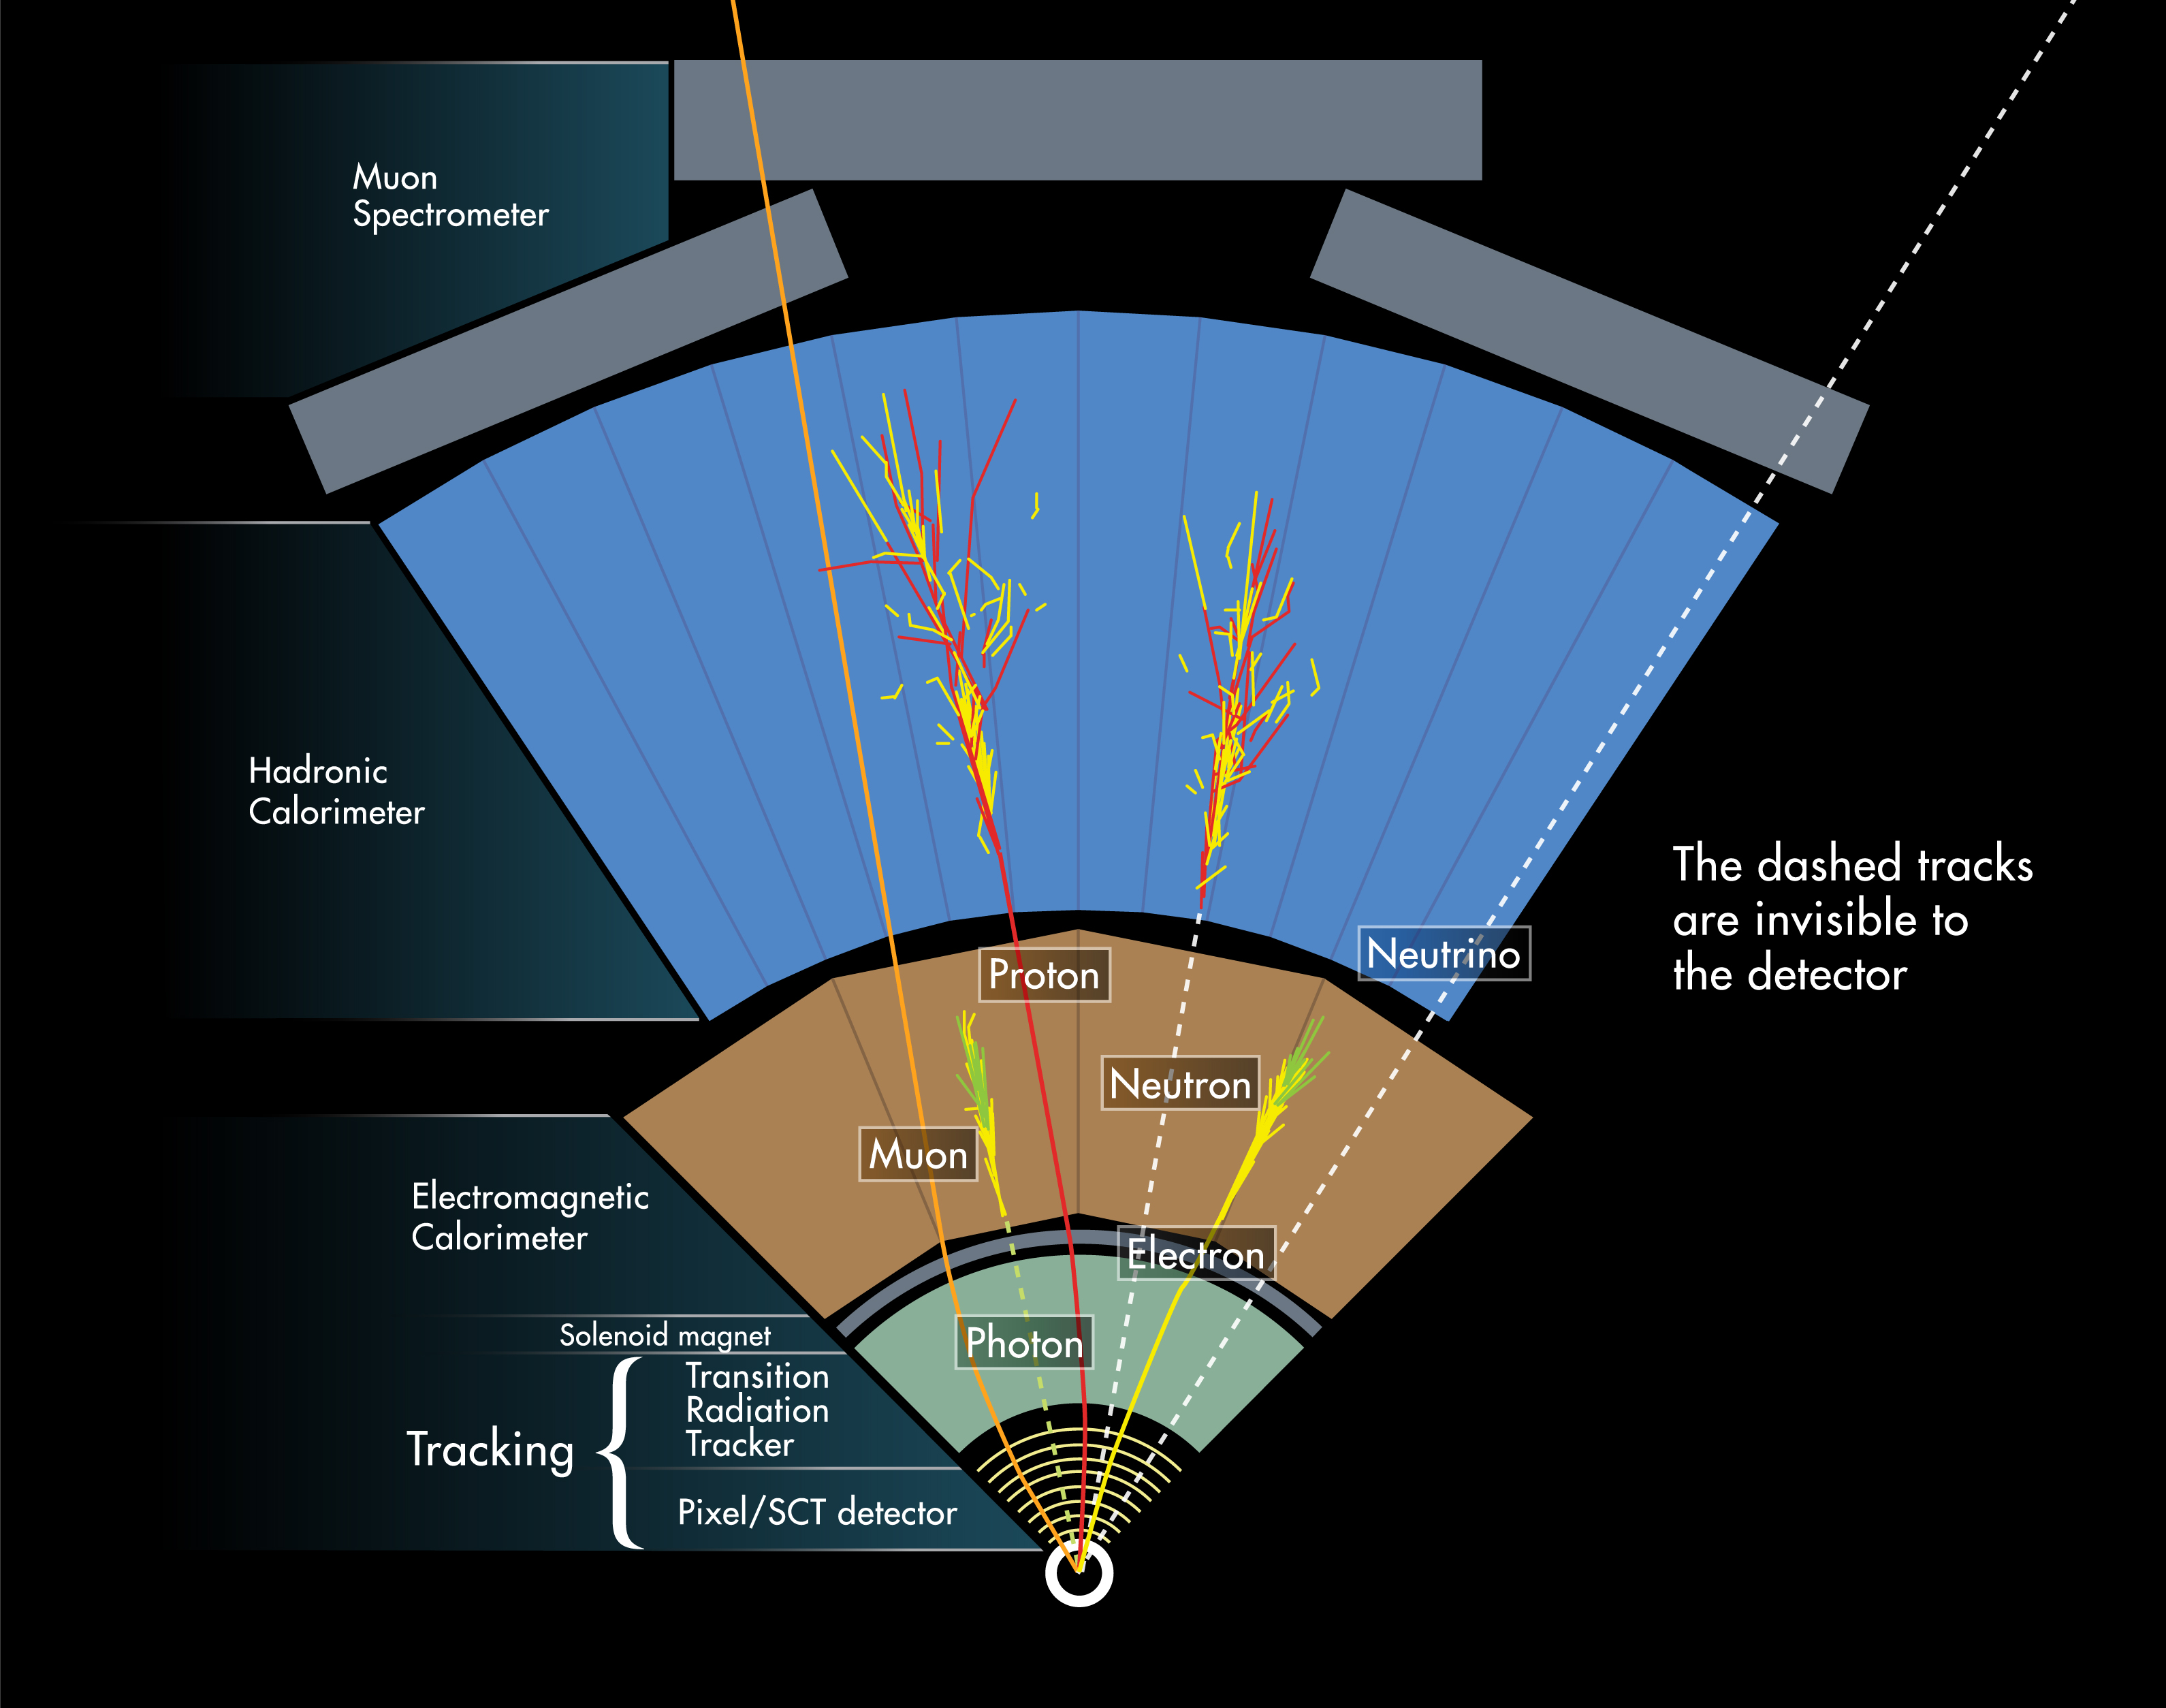
\includegraphics[width=1.0\textwidth]{EVENTRECO/ATLASOBJECTS.jpg}
     \caption{
         Illustration of a section of the~\acrshort{ATLASlabel} detector showing the interaction of particles with the different sub-detectors~\cite{Pequenao:1505342}. 
     }
     \label{figEVNTRECO:ATLASOBJECTS}
     \end{center}
 \end{figure}

\clearpage

\section{Basic objects}

The fundamental blocks used in the reconstruction algorithms are tracks, vertices and topo-clusters (or calorimeter energy clusters). All physics objects are composed by these blocks and introduced in the following section.

\subsection{Tracks and vertices}

Tracks are reconstructed objects produced by charged particles interacting in the \acrshort{IDlabel} and \acrshort{MSlabel} and used to identify their trajectory. The reconstruction consists in grouping hits from the different tracking sub-systems and requiring different criteria to ensure the quality of the tracks. The tracks that originate from the hard-scattering are referred to as primary tracks, and the origin of the track (vertex) is referred to as the \acrfull{PVlabel}.\\

As a first step, hits are built from groups of pixels and strips that reach a threshold energy deposit. Starting from the inner~\acrshort{IDlabel} layers, the seed to reconstruct a track consists of three hits in the silicon detector, and then hits from the outer layers of the tracker are added iteratively if compatible with the trajectory. When adding hits, a score is assigned to the track to quantify the correctness of the track trajectory and suppresses the contribution of random collections of hits (or fake tracks). Then, a dedicated algorithm evaluates the different seeds to limit shared hits, which typically indicate wrong assignments. In addition, quality criteria are applied: tracks are required to have $\pT>500$~MeV, $\abs{\eta}<2.5$, a minimum of seven pixel and \acrshort{SCTlabel} clusters, a maximum of either one shared pixel or two \acrshort{SCTlabel} clusters on the same layer, no more than one missing expected hit (or hole) in the pixel detector and a maximum of two holes in both pixel and \acrshort{SCTlabel} clusters. Also, the transverse impact parameter calculated with respect to the beam position, $\abs{d_0}$, is required to be smaller than 2~mm. In addition, the longitudinal difference between the \acrshort{PVlabel} and $d_0$ along the beam, $\abs{z_0 \sin\theta}$, is requiered to be smaller than 3~mm. As a last step, \acrshort{TRTlabel} hits are added to the tracks after extrapolation.\\

Vertices are of particular interest as they are the origin of the charged particles or interactions. The \acrshort{PVlabel} is the most important one, as it denotes the origin of the hard-scattering interaction, but secondary vertices are also characteristic of the origin of heavy-quarks or long-lived particles.\\

For a given event, the \acrshort{PVlabel}s are reconstructed iteratively from tracks using a dedicated vertex finding algorithm. From a set of quality tracks, a candidate position is defined and the compatibility with the set of tracks in terms of weights is evaluated in order to recompute the vertex position. In each step then, the tracks that are less compatible are given smaller weights and, after the convergence of the optimal vertex position, are left unassigned and remain as input for the following vertex. The \acrshort{PVlabel} is defined as the vertex with the largest $\pT^2$ sum. 

\subsection{Topological clusters}

Topological cell clusters, or topo-clusters, are objects reconstructed iteratively from calorimeter information. The signal is from the energy deposited in the different calorimeter cells by particle showers. The seed of a topo-cluster consists of calorimeter cells whose readout signal is four times higher than the background noise, and neighbouring cells are added if the ratio is higher than two. As a last step, an extra layer is added regardless of the signal-to-background ratio. This clustering takes advantage of the high granularity of the calorimeters and the resulting objects are used for the reconstruction of electrons, photons and hadrons.

\section{Jets}

Jets are cone-shaped collimated showers formed by the hadronic cascades that originate from the complex interactions of quarks and gluons when travelling through the detector. These objects are essential for physics analyses with partons in the final state, especially $b$-quarks, whose jets have particular properties that can be used to characterise them with great efficiency. Nevertheless, the kinematic properties of the cascades are challenging to define, as they can contain information from one or multiple final state partons and from the hard-scattering or other radiation processes.\\

There are different possible definitions that depend of dedicated algorithms which group calorimeter information and do not depend on common \acrshort{QCD} effects. Jet algorithms are collinear safe, referred to the jet configuration not changing if two constituents are merged forming one with double the momentum (or vice-versa), and infrared safe, meaning that the reconstruction is not affected by adding low \pT\ particles.

\subsection{Reconstruction}

The jet reconstruction is typically performed combining four-vector objects using the anti-k$_t$ algorithm~\cite{Cacciari_2008}. The algorithm merges clusters based on a relative distance defined as,

\begin{equation}
    d_{i,j} = \min (p_{\text{T},i}^{2n},p_{\text{T},j}^{2n}) \frac{\Delta R_{i,j}}{R^2}
\end{equation}

with $p_{\text{T},i/j}$ being the \pT\ of the cluster $i$ and $j$, $\Delta R_{i,j}$ the angle separation between them, $R$ the chosen radius parameter that sets the size of the jet and $n$ the chosen integer that defines the \pT\ dependence of $d_{i,j}$. The decision to combine clusters or to define a cluster as a jet comes from comparing the $d_{i,j}$ value with the beam spot distance, $d_{i,B} = p_{\text{T},i}^{2n}$. Clusters are grouped if $d_{i,j} < d_{i,B}$, otherwise the cluster $i$ is defined as a jet, in an iterative process until all input clusters are used. The anti-k$_t$ algorithm is defined by setting $n=-1$, which groups with higher priority the high energy clusters, and leads to a cone-shape around the highest object. This feature can be observed in Figure~\ref{figEVNTRECO:antikt}.\\

\begin{figure}[htbp]
    \RawFloats
    \begin{center}
    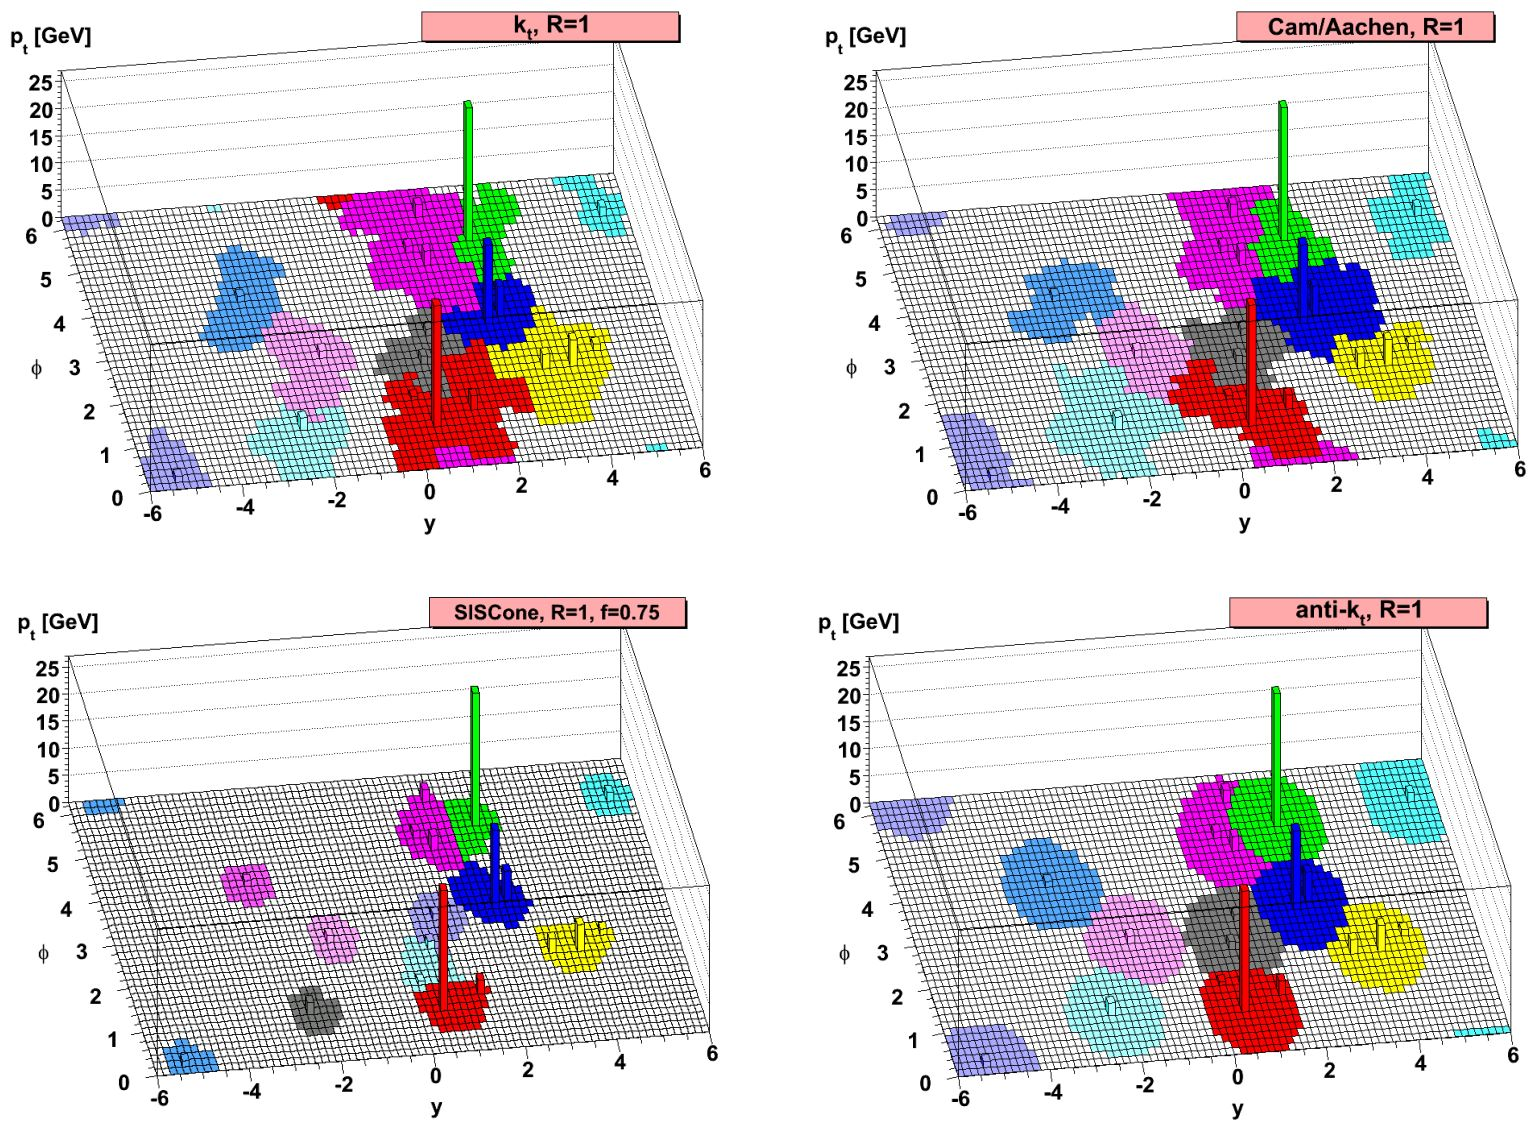
\includegraphics[width=1.0\textwidth]{EVENTRECO/antikt.JPG}
    \caption{
        Illustration of different clustering algorithms. The anti-k$_t$ (bottom right) shows cone-like structure around the track with the highest momentum~\cite{Cacciari_2008}. 
    }
    \label{figEVNTRECO:antikt}
    \end{center}
\end{figure}

Various definitions of jets are used in \acrshort{ATLASlabel}. In this thesis, EMTopo jets and PFlow jets are used and described in the following.

\subsubsection{EMTopo jets}

The so-called EMTopo jets are the primary jet definition used in physics analyses in \acrshort{ATLASlabel} before the end of Run~2. The reconstruction is performed at the EM energy scale only using topo-clusters~\cite{PhysRevD.96.072002} with the anti-k$_t$ algorithm implemented in the \textit{FASTJET} software package~\cite{Cacciari2012}. The jets used in this thesis are reconstructed with the radius parameter $R = 0.4$ with requirements in $\pT > 25$~GeV and $\abs{\eta} < 2.5$. The EMTopo jets are calibrated in several steps, summarised in Figure~\ref{figEVNTRECO:EMTOPO} and described below.\\

After the jet reconstruction, the jet direction is modified such that the jet originates from the primary vertex. Then, energy corrections based on pile-up are applied subtracting the average energy due to in-time pile-up and other residual corrections that depend on the number of \acrshort{PVlabel}; and bunch crossings. After, absolute calibrations are applied to the \acrlong{JESlabel}~(\acrshort{JESlabel}) and $\eta$ derived from dedicated dijet \acrshort{MClabel} events. Then, a global sequential calibration is applied to improve the \pT\ resolution and the associated uncertainties from the jet fluctuations that can arise from various initial factors, like the flavour or energy of the original parton. The final step is the in-situ calibration, which is only applied to data and is extracted from jets \pT and $\eta$ comparisons of data to known well-modelled \acrshort{MClabel} that include central jets in dijet events, $\gamma/Z+jets$ or multijet events.\\

\begin{figure}[htbp]
    \RawFloats
    \begin{center}
    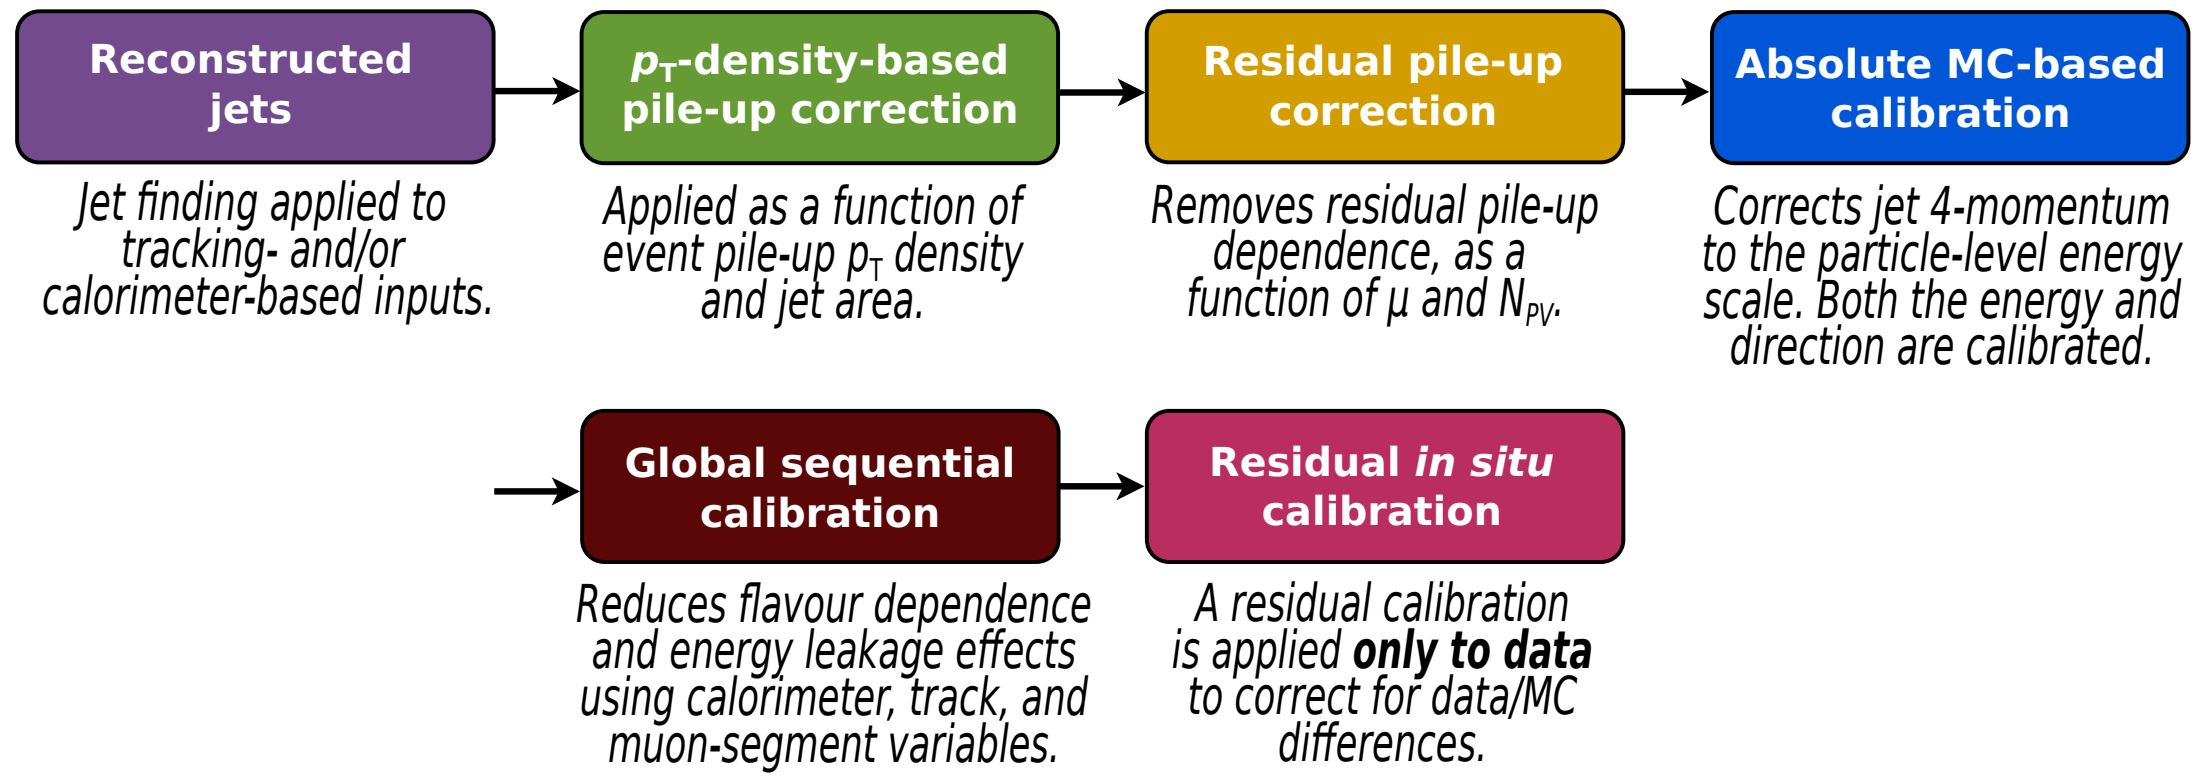
\includegraphics[width=1.0\textwidth]{EVENTRECO/EMTOPOCALIB.JPG}
    \caption{
        Stages of jet energy scale calibrations, all applied to the four-momentum of the jet~\cite{2007.02645}. 
    }
    \label{figEVNTRECO:EMTOPO}
    \end{center}
\end{figure}
\subsubsection{PFlow jets}

Particle Flow jets, known as PFlow jets, were introduced during Run~2 and combine tracking and calorimeter information. This type of jets has improved energy and angular resolution compared to EMTopo jets and enhanced reconstruction and stability against pile-up.\\

The reconstruction~\cite{pflow} is also based on the anti-k$_t$ algorithm with $R=0.4$, and the first step consists in matching the tracks (from the \acrshort{IDlabel}) from charged particles to the topo-clusters. The energy deposits of the matched topo-clusters are replaced by the corresponding track momentum. Then, the resulting topo-clusters and the tracks matched to the \acrshort{PVlabel} are used as input to the anti-k$_t$ algorithm. The jets are calibrated like the EMTopo jets in the range $20\text{ GeV}<\pT<1500$~GeV~\cite{ATLAS_Collaboration2020-ip}. 

\subsection{Jet tagging}

Jet or flavour tagging consists in identifying the parton flavour that generated the signal reconstructed as a jet. Efficient tagging is essential for analyses studying processes with $b$- or $c$-quarks in their final state (knows as heavy flavour quarks), as the jet tagging is additional information that can be used to select events with various jets and improves the signal efficiency.\\

Jets originating from the hadronisation of $b$-quarks, or $b$-tagged jets, leave a distinct signal due to the properties of $b$-hadrons: lifetime of $\sim$10$^{-12}$~s ($b$'s with $\pT>30$~GeV decay after 2.5~mm), mass of $\sim$5~GeV and high decay multiplicity (including semi-leptonic decays). Figure~\ref{figEVNTRECO:BTAGTOPO} shows a scheme of a typical signal, that includes displaced tracks with large $d_0$.\\

The signal of the $c$-hadrons is similar but not identical as the lifetime, mass and decay multiplicity are lower, which makes the distinction between these two kinds of jets difficult. The last type of jet is referred to light-flavour jets, whose signal originates directly from quark fragmentation and can be easily separated from $b$-jets. However, other phenomena like long-lived particles, photon conversions or low quality tracks can also prompt displaced vertices and tracks.

\begin{figure}[htbp]
    \RawFloats
    \begin{center}
    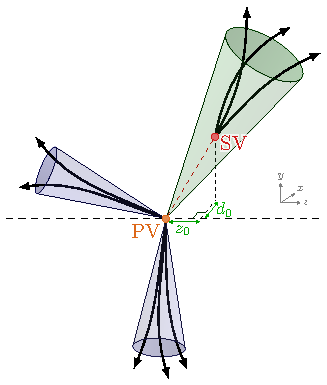
\includegraphics[width=0.75\textwidth]{EVENTRECO/btagdoodle.pdf}
    \caption{
        Schematic view of the typical topology of an event with a $b$-jet, including the~\acrshort{PVlabel}, a \acrlong{SVlabel}~(\acrshort{SVlabel}) with displaced tracks and the characteristic impact parameters, $d_0$ and $z_0$.
    }
    \label{figEVNTRECO:BTAGTOPO}
    \end{center}
\end{figure}

\subsubsection{Algorithms}

Flavour tagging algorithms use the properties of a given jet and return a score, referred to as output discriminant, which indicates how likely the input jet is considered to be a $b$-, $c$- or light-jet. Two algorithms are used in this thesis: the MV2c10 tagger which was the default option for EMTopo jets, and the DL1r tagger that is used for PFlow jets.\\

The MV2c10 tagger~\cite{ATL-PHYS-PUB-2015-022} is based on the MV2 algorithm, which relies on boosted decision trees~(BDTs) trained using several kinematic variables of the jets, properties of the secondary vertices and other taggers as inputs. The MV2c10 tagger was trained with \ttbar\ and $Z'$ events, to cover a large \pT\ spectrum, and $b$-jets defined as signal while the background consisted of 7\% $c$-jets and 93\% light-jets.\\

The DL1r tagger~\cite{taggingeff} is a multi-class Deep Neural Network (DNN) model, with three output nodes corresponding to the classification of the input jet to be a $b$-, $c$- or light jet. The final discriminant is given as a function of the three probabilities. The input to the training consists in the same inputs used for the MV2c10 tagger, additional variables for $c$-jet identification used in a jet vertex finder algorithm and flavour probabilities provided by a recursive NN designed to exploit the correlations between the tracks originating from the same $b$-hadron. The training set consists of the same \ttbar\ and $Z'$ events, weighted to have an equal mix of quark flavour jets.\\

The $b$-jet efficiency as a function of the jet \pT\ and the $c$- and light-jets rejection as a function of the jet $b$-jet efficiency for both MV2c10 and DL1r algorithms are shown in Figure~\ref{figEVNTRECO:taggingeff}. The DL1r tagger relies on more advanced machine learning techniques than the MV2c10 tagger. The multi-class output together with the possibility of tuning the final discriminant computation makes the DL1r tagger more flexible than the binary classification of MV2c10. Regarding performance, the efficiency of both algorithms to tag true $b$-jets is comparable, while the rejection rates of $c$- and light jets is larger for the DL1r tagger. The improvement in rejection for the 60\% working point, detailed below, is by up to 70\% for $c$-jets and 120\% for light jets.

\begin{figure}[htbp]
    \RawFloats
    \begin{center}
        \subfloat[]{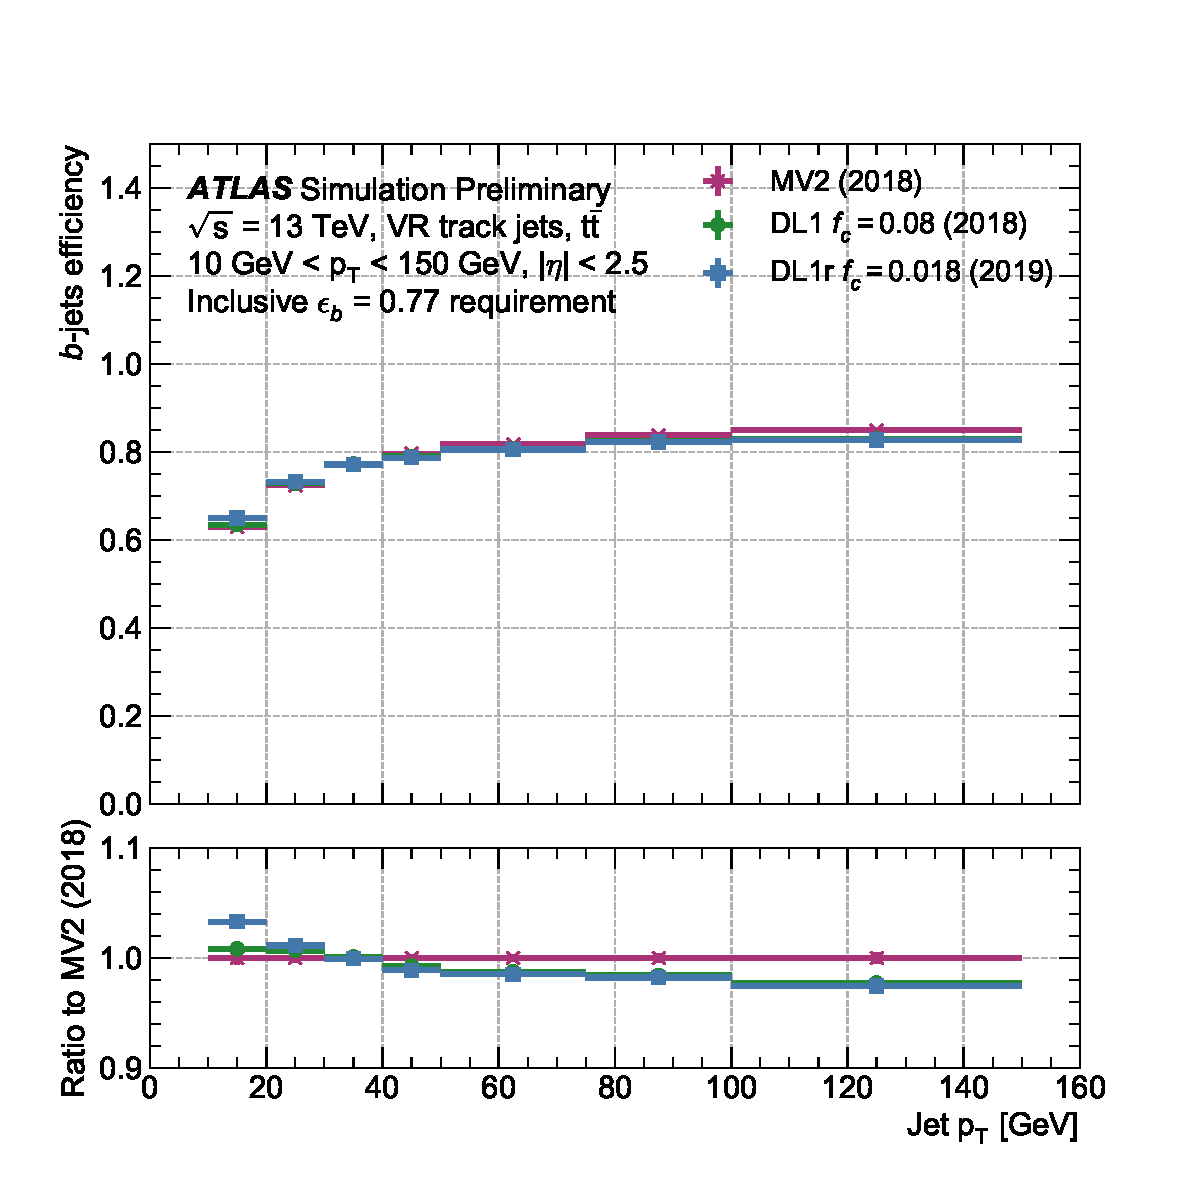
\includegraphics[width=0.47\textwidth]{EVENTRECO/btageff.pdf}} \\
        \subfloat[]{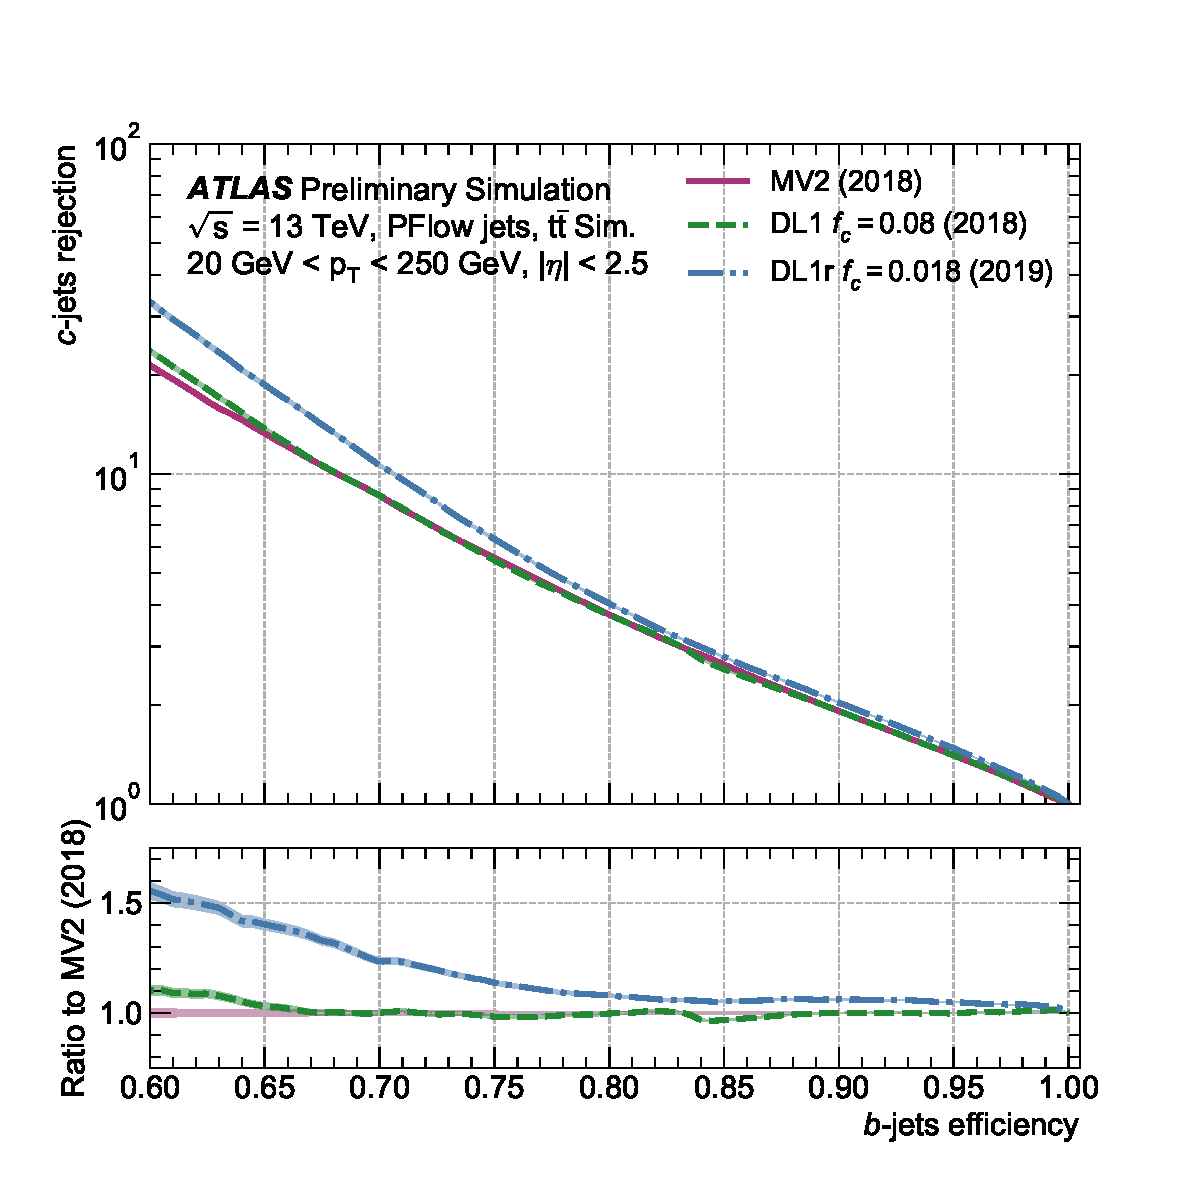
\includegraphics[width=0.47\textwidth]{EVENTRECO/ctagrej.pdf}}
        \quad
        \subfloat[]{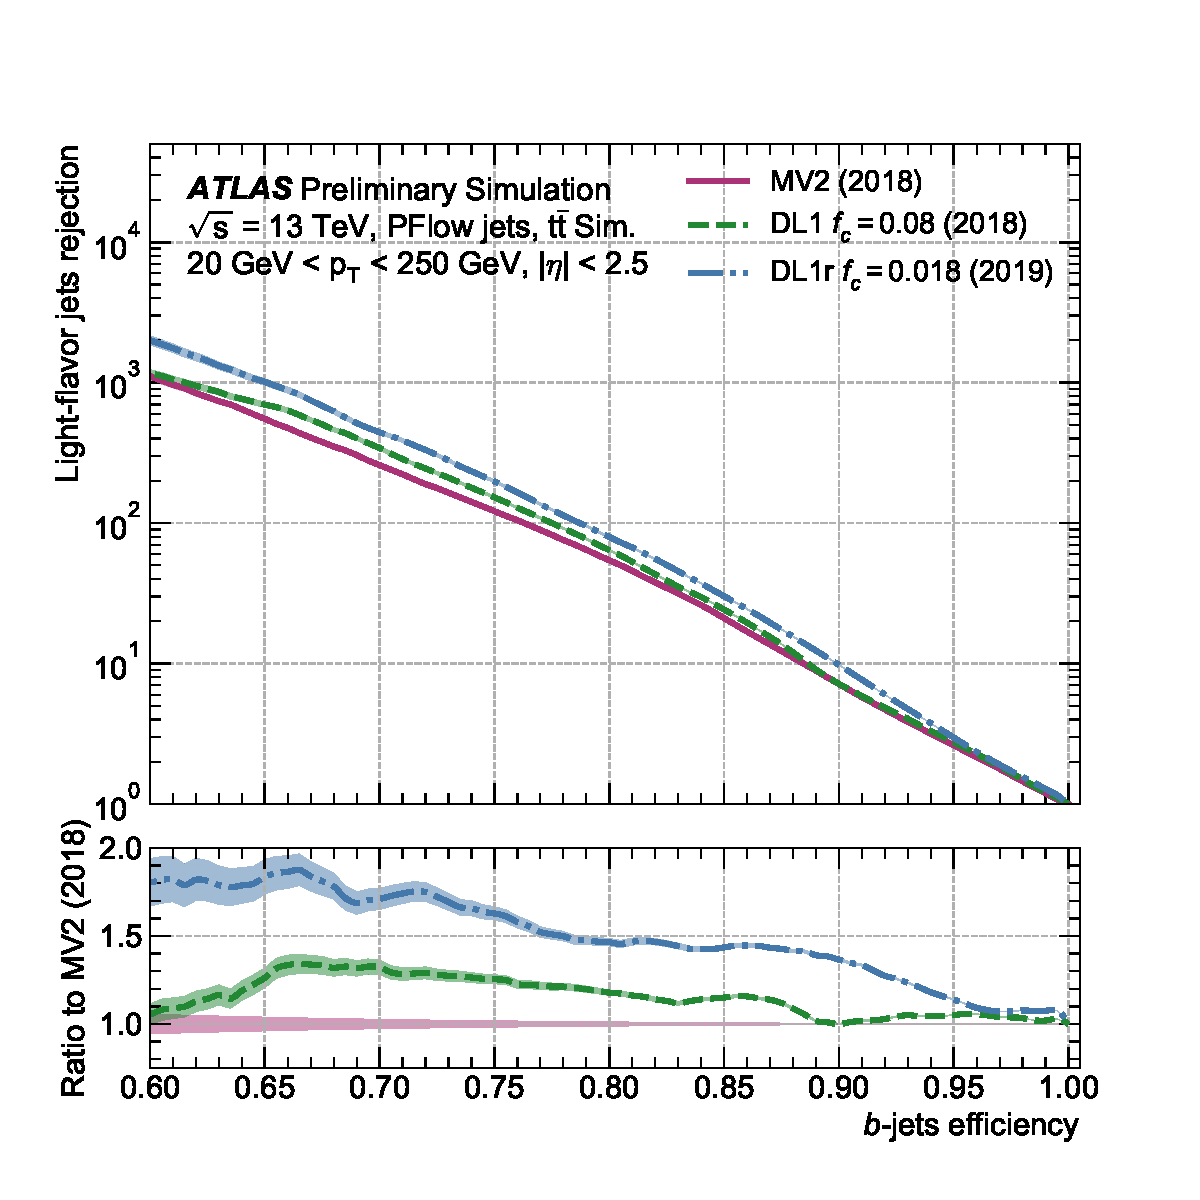
\includegraphics[width=0.47\textwidth]{EVENTRECO/ltagrej.pdf}}
        \caption{
        Identification efficiency for $b$-jets as a function of \pT\ (a), and rejection rate for $c$-jets (b) and light-jets (c) as a function of the $b$-tagging efficiency for the MV2c10 and DL1 taggers in a simulated \ttbar sample~\cite{taggingeff}.
    }
    \label{figEVNTRECO:taggingeff}
    \end{center}
\end{figure}

\subsubsection{Working points}

The full spectrum of the final $b$-tagging discriminant is not directly used in physics analyses due to the complexity of the calibration. Instead, four different $b$-tagging \acrlong{WPlabel}~(\acrshort{WPlabel}) are defined based on the $b$-jet acceptance efficiency evaluated on a \ttbar\ sample: 60\%, 70\%, 77\% and 85\%, which are often referred to as \textit{Very Tight}, \textit{Tight}, \textit{Medium} and \textit{Loose} operating points, respectively. Some $c$- and light-jets pass the 85\% \acrshort{WPlabel}, ending up with a $b$-tagging efficiency between 85\% and 100\%. Meanwhile, the jets that pass the 60\% \acrshort{WPlabel} mainly consists in $b$-jets.\\

The criteria are important when defining the $b$-jets for event selection, as the $b-$jets misidentification, so $c$- and $light$-jet acceptance inefficiency, improves for lower $b$-jet efficiency working points, therefore rejecting more background but with lower signal statistics. On the other hand, the pseudo-continuous b-tagging \acrshort{WPlabel}, so the \acrshort{WPlabel} that a jet passes, is additional information that can be used to further refine the selection or in multivariate methods.

\clearpage
\section{Leptons}

\subsection{Electrons}

Electrons interact with the \acrshort{IDlabel} and the \acrshort{EMlabel} calorimeter system. The typical signature is a track in the \acrshort{IDlabel} and electromagnetic shower in the \acrshort{EMlabel} calorimeter. Overall, the performance in terms of identification and reconstruction of electrons is high.\\

First, topo-clusters are selected and matched to \acrshort{IDlabel} tracks in the region $\abs{\eta}$ < 2.47 excluding the transition region of the barrel and end-cap (1.37 < $\abs{\eta}$ < 1.52). Next, the matched clusters are grouped to form superclusters, which are variable-size clusters, using a dynamic clustering algorithm. After a first energy and position calibration, tracks are matched to the electron superclusters. The calibration of the energy scale and resolution of electrons is computed from $Z\rightarrow ee$ decays and validated in $Z\rightarrow \ell\ell\gamma$~\cite{performanceEgamma}. In addition, the energy resolution of the reconstructed electron is optimised using a multivariate algorithm based on the properties of showers in the \acrshort{EMlabel} calorimeter.\\

Further identification criteria are required for an electron candidate, passing a selection to increase the purity. The prompt electrons are evaluated with a likelihood discriminant to define three operating points with different purities: \textit{Tight}, \textit{Medium} and \textit{Loose}. The discriminant is computed using variables measured in the \acrshort{IDlabel} and the \acrshort{EMlabel} calorimeter, chosen such that they discriminate prompt isolated electrons from other signal deposits (jets, converted photons or other electrons from heavy-flavoured hadron decays). The most important quantities are based on the track quality, the lateral and longitudinal development of the electromagnetic shower as well as the particle identification in the \acrshort{TRTlabel}. The probability density function to build the likelihood are derived from $Z\rightarrow ee$ ($E^\text{T}$ > 15~GeV) and $J/\psi \rightarrow ee$ ($E^\text{T}$ < 15~GeV) events.\\
%Figure 6.4 shows the data efficiency as a function of ET and as a function of the average number of bunch crossings for all three operating points. They are all optimised in 9 |eta| and 12 ET bins. 

Another requirement is the isolation criteria, to require the electron signal to be separated from other particles. Electrons are typically required to be spatially separated from other particles based on two quantities: a maximum value for the sum of transverse energy of topo-clusters in a $\Delta R=0.2$ cone surrounding the electron and of the sum of transverse momentum of tracks around the electron, with a $\Delta R$ cone that decreases with \pT. Effects of leakage and pile-up are taken into account and also tracks are required to satisfy \pT\ > 1~GeV, $\abs{\eta}<2.5$ and quality criteria. In this thesis, the criteria used is the Gradient isolation which has an efficiency of 90\% at $\pT = 25$~GeV and 99\% at $\pT = 60$~GeV.

\subsection{Muons}

Muons leave the \acrshort{ATLASlabel} detector without significant energy loss. The typical signal consists on a track in the \acrshort{IDlabel} and \acrshort{MSlabel} sub-detectors. There are different types of muons depending on which \acrshort{IDlabel}, \acrshort{MSlabel} or calorimeter information is available~\cite{performancemu}.\\

As a summary, the muon reconstruction has two stages: tracks are reconstructed independently in the \acrshort{IDlabel} and \acrshort{MSlabel}, and then are combined to form the muon tracks. The muon track candidates are built from track segments found in the different \acrshort{MSlabel} sub-systems. In the muon trigger chambers and \acrshort{MDTlabel}s, segments are reconstructed with a straight line to fit the hits of each detector layer after an alignment to the trajectory in the bending plane of the detector. The \acrshort{RPClabel}, \acrshort{TGClabel} and \acrshort{CSClabel} hits provide measurements in the orthogonal direction and the forward region of the detector to build additional track segments. The muon track candidates are then built from the track segments fit together using a global $\chi^2$ fit. With that information, different types of muons can be defined.\\

The combined (CB) muons are the muon candidates obtained from using combined information from \acrshort{MSlabel} tracks that are extrapolated to the tracks of \acrshort{IDlabel} (an inside-out approach is also used). The segment-tagged (ST) muons are reconstructed from tracks in the \acrshort{IDlabel} extrapolated to typically one track segment in the \acrshort{MDTlabel}s and \acrshort{CSClabel}. ST muons are normally low in \pT\ and in regions with low acceptance. Calorimeter-tagged (CT) muons are built from an \acrshort{IDlabel} track that is instead matched to an energy deposit in the calorimeter compatible with a minimal ionising particle. The CT muon strategy outputs the lowest purity, although proves useful for detector regions not fully covered by the \acrshort{MSlabel}, and is optimised for 15~GeV < \pT\ < 100~GeV and $\abs{\eta}<0.1$. The fourth type, extrapolated (ME) muons, are only reconstructed using the \acrshort{MSlabel} with an acceptance of $2.5 < \abs{\eta} < 2.7$.\\

The muon identification criteria (similar to the electron identification) is performed applying quality criteria to increase the purity of the selection. In order to identify prompt muons with high efficiency and a
good momentum resolution, a requirement is done for the amount of hits in the \acrshort{IDlabel} and the \acrshort{MSlabel} systems. Four different muon operating points are defined: \textit{Tight}, \textit{Medium}, \textit{Loose}, \textit{high \pT} and \textit{low \pT}. The Medium and Loose working points are used in this thesis. The first one is widely used in physics analyses and is designed to minimise muon reconstruction and calibration systematic uncertainties. It consists of combined and extrapolated muons with three or more hits in at least two of the \acrshort{MDTlabel} layers, or just one hit for $\abs{\eta}<0.1$ with no more than one hole in the \acrshort{MSlabel}. On the other hand, the Loose working point maximises the reconstruction efficiency and accounts all types of muons, adding the segmented- and calorimeter-tagged muons for $\abs{\eta}<0.1$. The reconstruction efficiency for muons with \pT > 20~GeV at the Medium and Loose working points is 96.1\% and 98.1\%, respectively. \\

The isolation criteria is based on track and calorimeter variables, similar to the electron case. The criteria improve the efficiency removing non-prompt muons, the ones not generated in the hard-scattering but in other parton shower processes for example, which are usually close to jets and other objects. The track related variable, \pT$^{\text{varcone30}}$ is the scalar \pT\ sum of the additional tracks in a cone $\Delta R=10$~GeV$/\pT^\mu$ (maximum of 0.3), that depends on the muon transverse momentum $\pT^\mu$. The calorimeter related variable is the same as for electrons, built from the sum of energies around the muon track. In this thesis, the \textit{FixedCutTightTrackOnly} working point is used, which is defined only with track isolation: $\pT^\text{varcone30}/\pT^\mu<0.06$.       

\subsection{Taus}

The $\tau$ leptons typically decay before reaching active electronics of the \acrshort{ATLASlabel} detector and have to be identified via their decay products. The decay can be either leptonically (into electrons or muons) or hadronically. The leptonic decay represents the 35\% of the cases and is covered by the reconstruction of the produced electron or muon. The hadronic decays represent 65\%, which contain one or three charged pions in 72\% and 22\% of the cases, respectively. In addition, at least one associated neutral pion is also produced in 68\% of the hadronic decays. The dedicated $\tau$ reconstruction and identification algorithms in \acrshort{ATLASlabel} target the hadronic decay, with the main background being jets from energetic hadrons produced in the fragmentation of quarks and gluons, known as the \acrshort{QCD} background. Therefore, the $\tau$ objects in \acrshort{ATLASlabel} mentioned in this thesis refer to hadronically decaying $\tau$ leptons. \\

The candidates are seeded by jets which are required to have $\pT > 10$~GeV and $\abs{\eta} < 2.5$ excluding the barrel-end-cap transition region~\cite{ATLAS-CONF-2017-029}. The tau identification is based on a machine learning classifier which is trained using the calorimeter information and the tracks associated to the jet candidate. A trained BDT is used for EMTopo jets while a recurrent NN is used for PFlow jets. Three different efficiency working points are defined: \textit{Loose
}, \textit{Medium} and \textit{Tight}. The $\tau$ leptons used in this thesis are defined with the medium working point, required to have $\pT>25$~GeV and isolation criteria of $\Delta R<0.2$ between the $\tau$ and any selected electron or muon.

\section{Missing transverse energy}

The missing transverse momentum, also denoted as \MET\ is the transverse component of the negative vector sum of the fully calibrated objects (electrons, muons, photons, $\tau$ leptons and jets) as well as soft objects associated to the \acrshort{PVlabel}. In an ideal detector, the the sum of four-momenta of all particles produced is equal to the net momentum of the initial collision, implying that the net momentum in the transverse plane of the collision has to be zero, $\MET=0$. Nevertheless, the net momentum is not null as particles like neutrinos leave the detector without depositing energy or others can interact with the detector in regions not covered by electronics. For analyses with neutrinos in the final state, it is typical to consider that the transverse energy carried by the neutrinos is the $\MET$, which allows their reconstruction.